% Options for packages loaded elsewhere
\PassOptionsToPackage{unicode}{hyperref}
\PassOptionsToPackage{hyphens}{url}
\PassOptionsToPackage{dvipsnames,svgnames,x11names}{xcolor}
%
\documentclass[
  letterpaper,
  DIV=11,
  numbers=noendperiod,
  oneside]{scrartcl}

\usepackage{amsmath,amssymb}
\usepackage{iftex}
\ifPDFTeX
  \usepackage[T1]{fontenc}
  \usepackage[utf8]{inputenc}
  \usepackage{textcomp} % provide euro and other symbols
\else % if luatex or xetex
  \usepackage{unicode-math}
  \defaultfontfeatures{Scale=MatchLowercase}
  \defaultfontfeatures[\rmfamily]{Ligatures=TeX,Scale=1}
\fi
\usepackage{lmodern}
\ifPDFTeX\else  
    % xetex/luatex font selection
\fi
% Use upquote if available, for straight quotes in verbatim environments
\IfFileExists{upquote.sty}{\usepackage{upquote}}{}
\IfFileExists{microtype.sty}{% use microtype if available
  \usepackage[]{microtype}
  \UseMicrotypeSet[protrusion]{basicmath} % disable protrusion for tt fonts
}{}
\makeatletter
\@ifundefined{KOMAClassName}{% if non-KOMA class
  \IfFileExists{parskip.sty}{%
    \usepackage{parskip}
  }{% else
    \setlength{\parindent}{0pt}
    \setlength{\parskip}{6pt plus 2pt minus 1pt}}
}{% if KOMA class
  \KOMAoptions{parskip=half}}
\makeatother
\usepackage{xcolor}
\usepackage[left=1in,marginparwidth=2.0666666666667in,textwidth=4.1333333333333in,marginparsep=0.3in]{geometry}
\setlength{\emergencystretch}{3em} % prevent overfull lines
\setcounter{secnumdepth}{-\maxdimen} % remove section numbering
% Make \paragraph and \subparagraph free-standing
\makeatletter
\ifx\paragraph\undefined\else
  \let\oldparagraph\paragraph
  \renewcommand{\paragraph}{
    \@ifstar
      \xxxParagraphStar
      \xxxParagraphNoStar
  }
  \newcommand{\xxxParagraphStar}[1]{\oldparagraph*{#1}\mbox{}}
  \newcommand{\xxxParagraphNoStar}[1]{\oldparagraph{#1}\mbox{}}
\fi
\ifx\subparagraph\undefined\else
  \let\oldsubparagraph\subparagraph
  \renewcommand{\subparagraph}{
    \@ifstar
      \xxxSubParagraphStar
      \xxxSubParagraphNoStar
  }
  \newcommand{\xxxSubParagraphStar}[1]{\oldsubparagraph*{#1}\mbox{}}
  \newcommand{\xxxSubParagraphNoStar}[1]{\oldsubparagraph{#1}\mbox{}}
\fi
\makeatother


\providecommand{\tightlist}{%
  \setlength{\itemsep}{0pt}\setlength{\parskip}{0pt}}\usepackage{longtable,booktabs,array}
\usepackage{calc} % for calculating minipage widths
% Correct order of tables after \paragraph or \subparagraph
\usepackage{etoolbox}
\makeatletter
\patchcmd\longtable{\par}{\if@noskipsec\mbox{}\fi\par}{}{}
\makeatother
% Allow footnotes in longtable head/foot
\IfFileExists{footnotehyper.sty}{\usepackage{footnotehyper}}{\usepackage{footnote}}
\makesavenoteenv{longtable}
\usepackage{graphicx}
\makeatletter
\newsavebox\pandoc@box
\newcommand*\pandocbounded[1]{% scales image to fit in text height/width
  \sbox\pandoc@box{#1}%
  \Gscale@div\@tempa{\textheight}{\dimexpr\ht\pandoc@box+\dp\pandoc@box\relax}%
  \Gscale@div\@tempb{\linewidth}{\wd\pandoc@box}%
  \ifdim\@tempb\p@<\@tempa\p@\let\@tempa\@tempb\fi% select the smaller of both
  \ifdim\@tempa\p@<\p@\scalebox{\@tempa}{\usebox\pandoc@box}%
  \else\usebox{\pandoc@box}%
  \fi%
}
% Set default figure placement to htbp
\def\fps@figure{htbp}
\makeatother

\usepackage{booktabs}
\usepackage{longtable}
\usepackage{array}
\usepackage{multirow}
\usepackage{wrapfig}
\usepackage{float}
\usepackage{colortbl}
\usepackage{pdflscape}
\usepackage{tabu}
\usepackage{threeparttable}
\usepackage{threeparttablex}
\usepackage[normalem]{ulem}
\usepackage{makecell}
\usepackage{xcolor}
\KOMAoption{captions}{tableheading}
\makeatletter
\@ifpackageloaded{caption}{}{\usepackage{caption}}
\AtBeginDocument{%
\ifdefined\contentsname
  \renewcommand*\contentsname{Table of contents}
\else
  \newcommand\contentsname{Table of contents}
\fi
\ifdefined\listfigurename
  \renewcommand*\listfigurename{List of Figures}
\else
  \newcommand\listfigurename{List of Figures}
\fi
\ifdefined\listtablename
  \renewcommand*\listtablename{List of Tables}
\else
  \newcommand\listtablename{List of Tables}
\fi
\ifdefined\figurename
  \renewcommand*\figurename{Figure}
\else
  \newcommand\figurename{Figure}
\fi
\ifdefined\tablename
  \renewcommand*\tablename{Table}
\else
  \newcommand\tablename{Table}
\fi
}
\@ifpackageloaded{float}{}{\usepackage{float}}
\floatstyle{ruled}
\@ifundefined{c@chapter}{\newfloat{codelisting}{h}{lop}}{\newfloat{codelisting}{h}{lop}[chapter]}
\floatname{codelisting}{Listing}
\newcommand*\listoflistings{\listof{codelisting}{List of Listings}}
\makeatother
\makeatletter
\makeatother
\makeatletter
\@ifpackageloaded{caption}{}{\usepackage{caption}}
\@ifpackageloaded{subcaption}{}{\usepackage{subcaption}}
\makeatother
\makeatletter
\@ifpackageloaded{sidenotes}{}{\usepackage{sidenotes}}
\@ifpackageloaded{marginnote}{}{\usepackage{marginnote}}
\makeatother

\usepackage{bookmark}

\IfFileExists{xurl.sty}{\usepackage{xurl}}{} % add URL line breaks if available
\urlstyle{same} % disable monospaced font for URLs
\hypersetup{
  pdftitle={Supply Chain Data Analytics},
  colorlinks=true,
  linkcolor={blue},
  filecolor={Maroon},
  citecolor={Blue},
  urlcolor={Blue},
  pdfcreator={LaTeX via pandoc}}


\title{Supply Chain Data Analytics}
\usepackage{etoolbox}
\makeatletter
\providecommand{\subtitle}[1]{% add subtitle to \maketitle
  \apptocmd{\@title}{\par {\large #1 \par}}{}{}
}
\makeatother
\subtitle{Analyzing and Forcasting Supermarket Sales}
\author{Stan Brouwer (2671939) \and Liz Chen (2840693) \and Maaike
Lamberts (2854979) \and Niek Schroor (2786837)}
\date{2024-12-11}

\begin{document}
\maketitle


\marginnote{\begin{footnotesize}

please visit https://sjbrou.github.io/Supply\_Chain\_Data\_Analysis/ for
an interactive version with better visualizations!

\end{footnotesize}}

\subsection{Data selection}\label{data-selection}

We analyze, forecast and interpret the
\href{https://public.tableau.com/app/sample-data/sample_-_superstore.xls}{Superstore
sales} provided by
\href{https://public.tableau.com/app/learn/sample-data}{Tableau} using
different statistical and machine learning methods.

The dataset provided contains information about products, sales and
profits of a fictitious US company. The dataset contains about 10,000
rows with 1,850 unique product names and 17 product subcategories,
covering four consecutive years on a daily basis.

We describe our work in the PDF version. However, we would like to
recommend reading our quarto manuscript \emph{here} as it contains the
\textbf{relevant} R code in the Article Notebook.

\subsection{Data Pre-processing}\label{data-pre-processing}

The superstore data set we selected is of high quality: At first glance
(which needs to be verified during the visualization), the data appears
to have been recorded regularly and without interruptions. There is no
sign of a sudden structural change. Since the data are consumer
products, it should contain both trends and seasonality. Nevertheless,
we have included hypothetical steps to demonstrate our understanding of
the data preprocessing procedure. In detail, we did:

\textsubscript{Source:
\href{https://SJbrou.github.io/Supply_Chain_Data_Analysis/index.qmd.html}{Article
Notebook}}

\begin{itemize}
\tightlist
\item
  Remove whitespaces from column names
\item
  Remove the Row\_ID column as it can be inferred by it's index
\item
  Remove all columns with a single unique value, as storing these would
  be
  \href{https://few.vu.nl/~molenaar/courses/StatR/chapters/B-06-raw_data.html}{redundant}
\item
  Ensure machine-readable date formats in yyyy-mm-dd as these usually
  differ per locale.
\item
  Ensure proper decimal separators
\item
  Calculate the number of missing values (both NA and empty string
  ``\,``) per column.
\end{itemize}

\textsubscript{Source:
\href{https://SJbrou.github.io/Supply_Chain_Data_Analysis/index.qmd.html}{Article
Notebook}}

After these steps (and transposing the table for better document
formatting), the data looks as follows:

\begin{longtable}[]{@{}
  >{\raggedright\arraybackslash}p{(\linewidth - 6\tabcolsep) * \real{0.0843}}
  >{\raggedright\arraybackslash}p{(\linewidth - 6\tabcolsep) * \real{0.2048}}
  >{\raggedright\arraybackslash}p{(\linewidth - 6\tabcolsep) * \real{0.3614}}
  >{\raggedright\arraybackslash}p{(\linewidth - 6\tabcolsep) * \real{0.3494}}@{}}
\caption{First 3 Rows of the Data (Transposed)}\tabularnewline
\toprule\noalign{}
\endfirsthead
\endhead
\bottomrule\noalign{}
\endlastfoot
Order\_ID & CA-2016-152156 & CA-2016-152156 & CA-2016-138688 \\
Order\_Date & 2016-11-08 & 2016-11-08 & 2016-06-12 \\
Ship\_Date & 2016-11-11 & 2016-11-11 & 2016-06-16 \\
Ship\_Mode & Second Class & Second Class & Second Class \\
Customer\_ID & CG-12520 & CG-12520 & DV-13045 \\
Customer\_Name & Claire Gute & Claire Gute & Darrin Van Huff \\
Segment & Consumer & Consumer & Corporate \\
City & Henderson & Henderson & Los Angeles \\
State & Kentucky & Kentucky & California \\
Postal\_Code & 42420 & 42420 & 90036 \\
Region & South & South & West \\
Product\_ID & FUR-BO-10001798 & FUR-CH-10000454 & OFF-LA-10000240 \\
Category & Furniture & Furniture & Office Supplies \\
Sub\_Category & Bookcases & Chairs & Labels \\
Product\_Name & Bush Somerset Collection Bookcase & Hon Deluxe Fabric
Upholstered Stacking Chairs, Rounded Back & Self-Adhesive Address Labels
for Typewriters by Universal \\
Sales & 261.96 & 731.94 & 14.62 \\
Quantity & 2 & 3 & 2 \\
Discount & 0 & 0 & 0 \\
Profit & 41.9136 & 219.5820 & 6.8714 \\
\end{longtable}

\textsubscript{Source:
\href{https://SJbrou.github.io/Supply_Chain_Data_Analysis/index.qmd.html}{Article
Notebook}}

We did not find any missing values, confirming the quality of the data
set. There is some more processing to do, for instance the removal of
outliers. However, by doing so we impose our own assumptions on the
data. Let's start by evaluating the descriptive statistics of our data
and check if further processing is required.

\textsubscript{Source:
\href{https://SJbrou.github.io/Supply_Chain_Data_Analysis/index.qmd.html}{Article
Notebook}}

\begin{longtable}[]{@{}llllll@{}}
\caption{Descriptive Statistics for Numeric Columns}\tabularnewline
\toprule\noalign{}
Column & Min & Max & Mean & Median & StdDev \\
\midrule\noalign{}
\endfirsthead
\toprule\noalign{}
Column & Min & Max & Mean & Median & StdDev \\
\midrule\noalign{}
\endhead
\bottomrule\noalign{}
\endlastfoot
Postal\_Code & 1040 & 99301 & 55190.38 & 56430.5 & 32063.69 \\
Sales & 0.444 & 22638.48 & 229.858 & 54.49 & 623.2451 \\
Quantity & 1 & 14 & 3.789574 & 3 & 2.22511 \\
Discount & 0 & 0.8 & 0.1562027 & 0.2 & 0.206452 \\
Profit & -6599.978 & 8399.976 & 28.6569 & 8.6665 & 234.2601 \\
\end{longtable}

\begin{longtable}[]{@{}lll@{}}
\caption{Descriptive Statistics for Date Columns}\tabularnewline
\toprule\noalign{}
Column & Earliest & Latest \\
\midrule\noalign{}
\endfirsthead
\toprule\noalign{}
Column & Earliest & Latest \\
\midrule\noalign{}
\endhead
\bottomrule\noalign{}
\endlastfoot
Order\_Date & 2014-01-03 & 2017-12-30 \\
Ship\_Date & 2014-01-07 & 2018-01-05 \\
\end{longtable}

\textsubscript{Source:
\href{https://SJbrou.github.io/Supply_Chain_Data_Analysis/index.qmd.html}{Article
Notebook}}

We inspect the orders with the lowest and highest Sales amount (in USD).
The most expensive orders were professional printers, cameras and
teleconferencing units with high unit prices. The orders with the lowest
sales amount were often binders and had a high Discount rate.

Interestingly there are orders with a negative profit. They typically
have high Discount rates and often concern the same item, such as the
``Cubify CubeX 3D Printer Triple Head Print''. The orders with a
negative Profit were often part of a larger order (for instance
CA-2016-108196), and placed by customers with multiple orders. We
suspect these negative Profit's to be caused by items of lower quality
that receive discounts, general discount codes, or volume discounts.
However, due to the high discounts especially on orders with negative
profit, we assume these to be valid orders.

** Some negative profit products **

In figure x we plotted the quantities of the most sold products.
Unfortunately, the sold quantities of individual products were too low
to determine any meaningful trends.

\textsubscript{Source:
\href{https://SJbrou.github.io/Supply_Chain_Data_Analysis/index.qmd.html}{Article
Notebook}}

\begin{figure}[H]

{\centering \pandocbounded{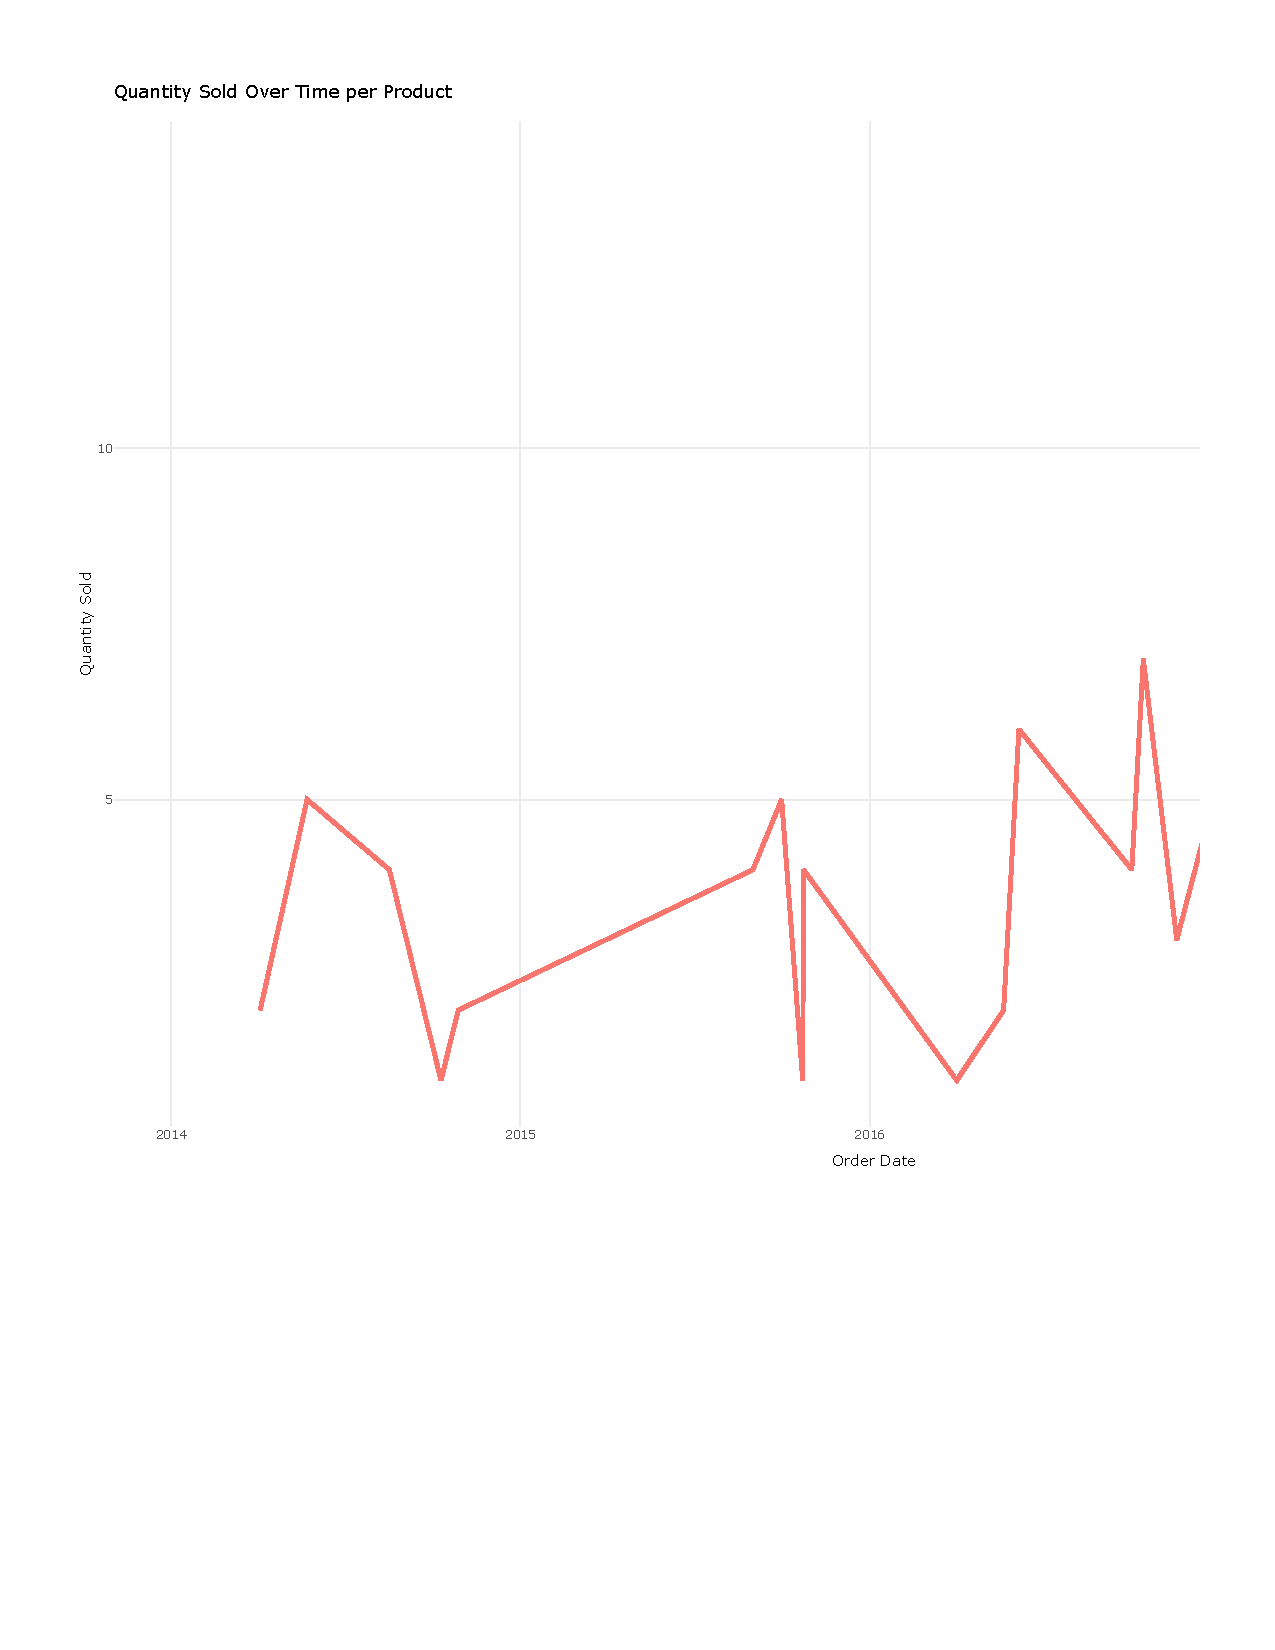
\includegraphics[keepaspectratio]{index_files/figure-pdf/Top_Products_Quantity-1.pdf}}

}

\caption{Figure X Sale quantity of the most popular products}

\end{figure}%

\textsubscript{Source:
\href{https://SJbrou.github.io/Supply_Chain_Data_Analysis/index.qmd.html}{Article
Notebook}}

Our proposed workaround is to aggregate Product\_Name by Sub\_Category,
and treat it as a single product for the rest of the assignment, which
we plotted in figure X.

\pandocbounded{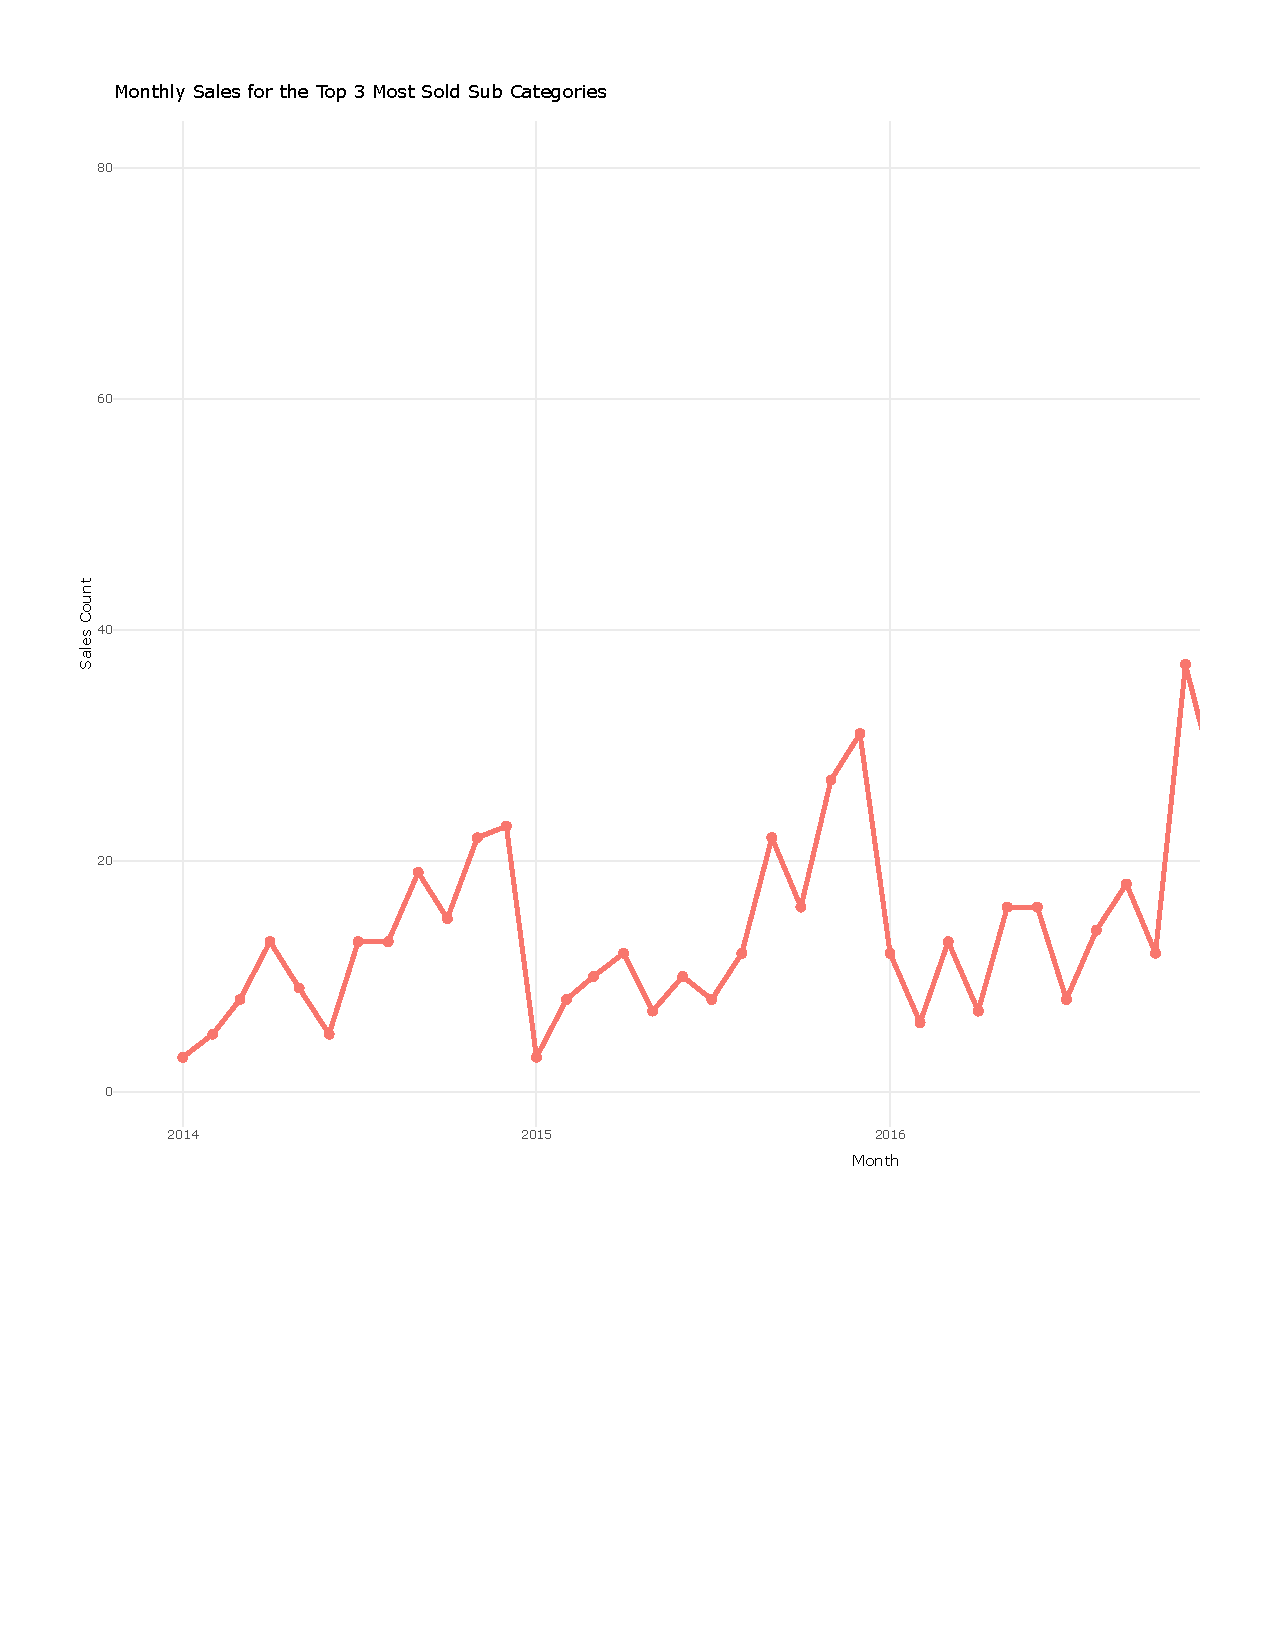
\includegraphics[keepaspectratio]{index_files/figure-pdf/Aggregated_Sub_Category_sales-1.pdf}}

\textsubscript{Source:
\href{https://SJbrou.github.io/Supply_Chain_Data_Analysis/index.qmd.html}{Article
Notebook}}

This aggregated Quantity starts to show trends and seasonality, and is
much more useful to base predictions on! We will use these aggregated
sub-categories for the rest of the assignment.

To properly finish our data preprocessing we ran some statistics on
Quantity aggregated by Sub\_Category. Table x contains some descriptive
statistics.

\begin{longtable}[]{@{}lrrrrrr@{}}
\caption{Statistics for Sub\_Category quantity}\tabularnewline
\toprule\noalign{}
Sub\_Category & Min & Mean & Max & Sd & CI\_lower & CI\_upper \\
\midrule\noalign{}
\endfirsthead
\toprule\noalign{}
Sub\_Category & Min & Mean & Max & Sd & CI\_lower & CI\_upper \\
\midrule\noalign{}
\endhead
\bottomrule\noalign{}
\endlastfoot
Accessories & 1 & 3.84 & 14 & 2.28 & 3.68 & 4.00 \\
Appliances & 1 & 3.71 & 14 & 2.12 & 3.52 & 3.90 \\
Art & 1 & 3.77 & 14 & 2.13 & 3.62 & 3.92 \\
Binders & 1 & 3.92 & 14 & 2.29 & 3.80 & 4.04 \\
Bookcases & 1 & 3.81 & 13 & 2.28 & 3.51 & 4.11 \\
Chairs & 1 & 3.82 & 14 & 2.28 & 3.64 & 4.00 \\
Copiers & 1 & 3.44 & 9 & 1.83 & 3.01 & 3.87 \\
Envelopes & 1 & 3.57 & 9 & 2.05 & 3.32 & 3.82 \\
Fasteners & 1 & 4.21 & 14 & 2.41 & 3.89 & 4.53 \\
Furnishings & 1 & 3.72 & 14 & 2.16 & 3.58 & 3.86 \\
Labels & 1 & 3.85 & 14 & 2.35 & 3.61 & 4.09 \\
Machines & 1 & 3.83 & 11 & 2.17 & 3.43 & 4.23 \\
Paper & 1 & 3.78 & 14 & 2.23 & 3.66 & 3.90 \\
Phones & 1 & 3.70 & 14 & 2.19 & 3.56 & 3.84 \\
Storage & 1 & 3.73 & 14 & 2.19 & 3.58 & 3.88 \\
Supplies & 1 & 3.41 & 10 & 1.84 & 3.15 & 3.67 \\
Tables & 1 & 3.89 & 13 & 2.45 & 3.62 & 4.16 \\
\end{longtable}

\textsubscript{Source:
\href{https://SJbrou.github.io/Supply_Chain_Data_Analysis/index.qmd.html}{Article
Notebook}}

The statistics for Quantity aggregated by Sub\_Category looks valid. We
can visualize it as histogram and check for anomalies. Figure y contains
histograms of Quantity per Sub\_Category.

\pandocbounded{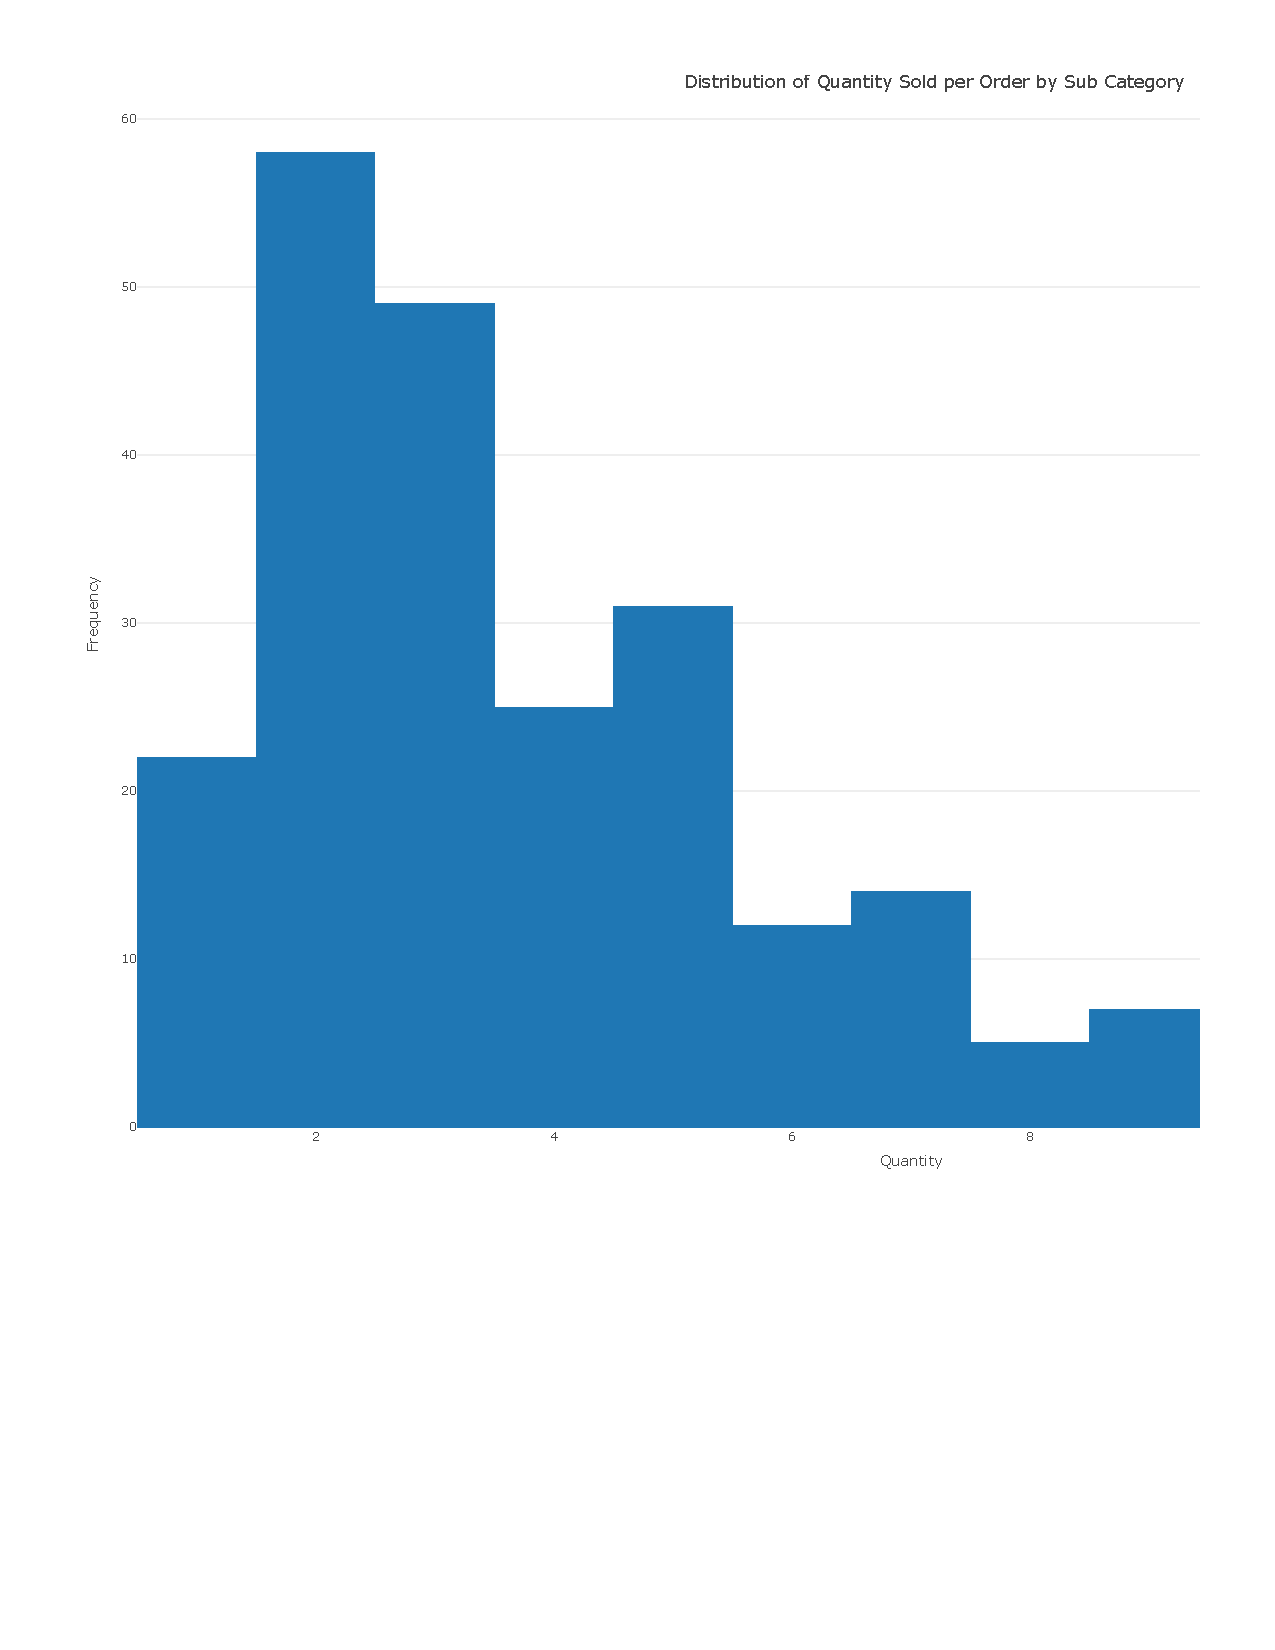
\includegraphics[keepaspectratio]{index_files/figure-pdf/sub_category_histograms-1.pdf}}

\textsubscript{Source:
\href{https://SJbrou.github.io/Supply_Chain_Data_Analysis/index.qmd.html}{Article
Notebook}}

The histograms show that the quantities a right-skewed distributed. This
is to be expected since most orders contain only a small number of
items. We will not remove the outliers with large quantities since they
appear valid..

\subsection{Forecasting Method
Evaluation}\label{forecasting-method-evaluation}

\subsubsection{Forecasting top 3 product categories
(4a)}\label{forecasting-top-3-product-categories-4a}

Let's forecast sold quantities for the three most sold sub-categories:

The steps taken for data preparation were:

\begin{itemize}
\tightlist
\item
  Identifying Top Subcategories: The top three subcategories are
  selected from our dataset based on their sold quantities. The top
  three were: Binders, furnishing and paper.
\item
  The sold quantities are aggregated monthly to create a time series
  object which we can use in the forecasting.
\item
  A KPSS showed that the data is non stationary. First-order
  differencing is applied to transform the data from non-stationary to
  stationary. The KPSS results in a p-value \textgreater0.05 showing the
  stationarity.
\end{itemize}

\textsubscript{Source:
\href{https://SJbrou.github.io/Supply_Chain_Data_Analysis/index.qmd.html}{Article
Notebook}}

Three models are applied to each subcategory to forecast it. The models
we use are: ARIMA, Holt-Winters and ETS. We have chosen these models
because of their level of suitability for discrete time series data with
all different levels of trend and seasonality. To evaluate the methods
and its effectiveness , the data is split into a training set (70\%) and
testing set (30\%).

\pandocbounded{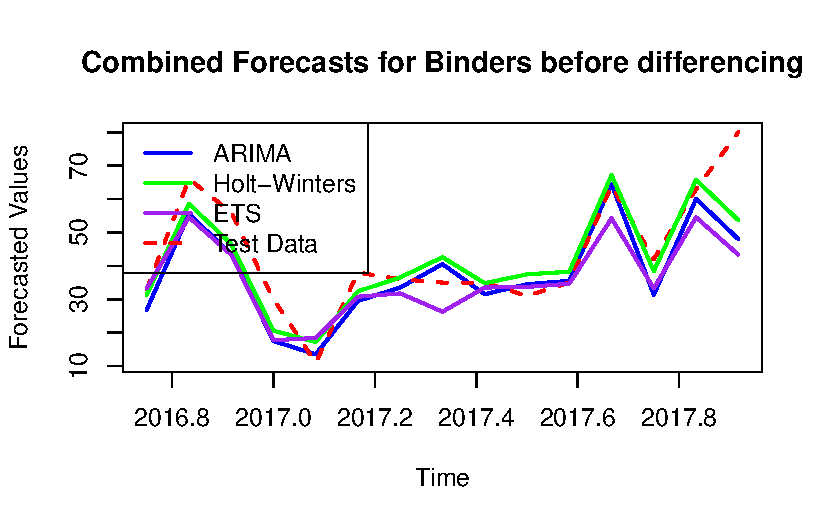
\includegraphics[keepaspectratio]{index_files/figure-pdf/Results1-1.pdf}}

\pandocbounded{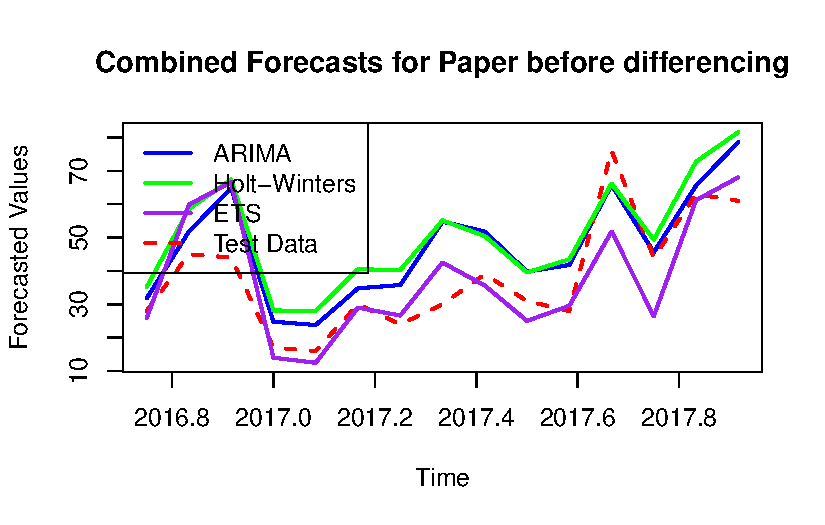
\includegraphics[keepaspectratio]{index_files/figure-pdf/Results1-2.pdf}}

\pandocbounded{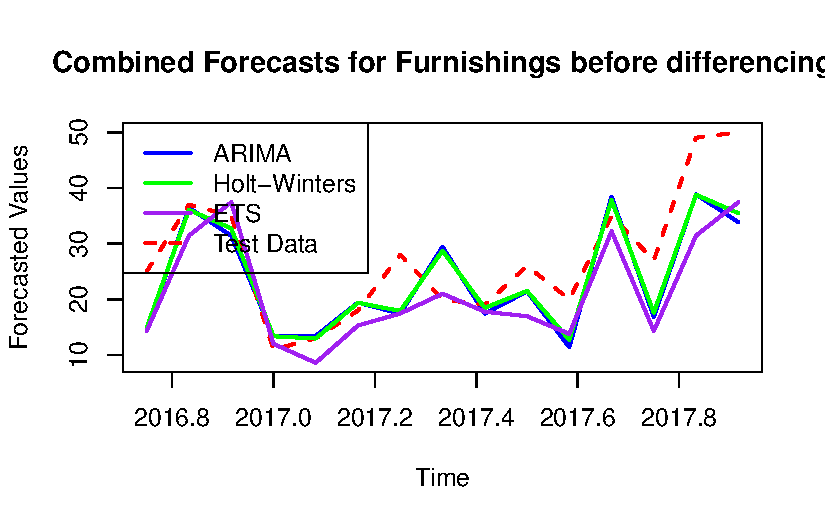
\includegraphics[keepaspectratio]{index_files/figure-pdf/Results1-3.pdf}}

\textsubscript{Source:
\href{https://SJbrou.github.io/Supply_Chain_Data_Analysis/index.qmd.html}{Article
Notebook}}

To assess the results, we use the following performance metrics: ME,
RMSE, MAE and MAPE. They are calculated for the training and testing
phases of the forecast.

\begin{longtable}[]{@{}llllrrrrrrrr@{}}
\caption{Training Set Forecast Accuracy}\tabularnewline
\toprule\noalign{}
& Sub\_Category & Method & Dataset & ME & RMSE & MAE & MPE & MAPE & MASE
& ACF1 & Theil\_U \\
\midrule\noalign{}
\endfirsthead
\toprule\noalign{}
& Sub\_Category & Method & Dataset & ME & RMSE & MAE & MPE & MAPE & MASE
& ACF1 & Theil\_U \\
\midrule\noalign{}
\endhead
\bottomrule\noalign{}
\endlastfoot
1 & Binders & ARIMA & Training set & 0.771 & 4.643 & 2.982 & 0.687 &
12.912 & 0.485 & 0.044 & NA \\
3 & Binders & HoltWinters & Training set & 0.867 & 5.215 & 3.790 &
-0.404 & 15.365 & 0.617 & -0.389 & NA \\
5 & Binders & ETS & Training set & 0.743 & 4.713 & 3.656 & 1.359 &
15.417 & 0.595 & -0.223 & NA \\
7 & Paper & ARIMA & Training set & 1.117 & 6.309 & 3.828 & 1.702 &
14.322 & 0.547 & -0.007 & NA \\
9 & Paper & HoltWinters & Training set & 1.510 & 7.280 & 4.855 & 3.325 &
16.413 & 0.694 & -0.027 & NA \\
11 & Paper & ETS & Training set & 0.609 & 6.205 & 4.475 & -1.662 &
18.732 & 0.639 & 0.005 & NA \\
13 & Furnishings & ARIMA & Training set & 0.005 & 3.874 & 2.568 & -6.625
& 20.210 & 0.556 & -0.202 & NA \\
15 & Furnishings & HoltWinters & Training set & 0.914 & 4.165 & 3.475 &
7.490 & 24.756 & 0.752 & -0.433 & NA \\
17 & Furnishings & ETS & Training set & 0.737 & 3.467 & 2.852 & 0.430 &
20.852 & 0.617 & -0.209 & NA \\
\end{longtable}

\textsubscript{Source:
\href{https://SJbrou.github.io/Supply_Chain_Data_Analysis/index.qmd.html}{Article
Notebook}}

As we can see on the forecasting results ARIMA performed well for
binders. We can state this because of the lowest RMSE.

For the subcategory furnishings we can see that the ETS forecasting
method is the most stable across the training and testing phase.

For the last subcategory and product paper the ETS model is again the
most consistent, comparing the statistics for training and test set. The
high variability in the test data leads to larger forecasting errors in
all the 3 models.

Concerning the residual diagnostics, the checks show no real
autocorrelation for ARIMA models. Which indicates a good fitting
forecast.

\subsubsection{Conclusion (4a)}\label{conclusion-4a}

The most effective model is not the same in all the subcategories. Each
model was validated based on its ability to capture seasonality and
trend. ARIMA performed better for Binders, while ETS performed better
for Furnishings and Paper.

\subsubsection{Clustering Subcategories and forecasting
(4b)}\label{clustering-subcategories-and-forecasting-4b}

Steps Taken:

\begin{itemize}
\tightlist
\item
  Trend strength, random variation and seasonal strength were calculated
  for the subcategory using the time series we have.
\end{itemize}

Clustering:

The clustering method used is the hierarchical clustering method. To
group subcategories into three different clusters based on features
which are normalized. The hierarchical clustering gave the following
results:

\begin{itemize}
\item
  Cluster 1: Stronger seasonality
\item
  Cluster 2: moderate trend and seasonality
\item
  Cluster 3: Lower trend and seasonal strength
\end{itemize}

For each different cluster we also used the models introduced in 4A
(ARIMA, Holt-Winters, ETS). These results where all aggregated at the
level of each cluster so we can assess mean RMSE and MAPE for each
different model.

\begin{longtable}[]{@{}llllrrrrrrrr@{}}
\caption{Forecast Accuracy Results}\tabularnewline
\toprule\noalign{}
& Sub\_Category & Method & Dataset & ME & RMSE & MAE & MPE & MAPE & MASE
& ACF1 & Theil\_U \\
\midrule\noalign{}
\endfirsthead
\toprule\noalign{}
& Sub\_Category & Method & Dataset & ME & RMSE & MAE & MPE & MAPE & MASE
& ACF1 & Theil\_U \\
\midrule\noalign{}
\endhead
\bottomrule\noalign{}
\endlastfoot
2 & Binders & ARIMA & Test set & 5.941 & 10.784 & 7.616 & 10.368 &
17.329 & 1.240 & 0.049 & 0.357 \\
4 & Binders & HoltWinters & Test set & 2.247 & 8.712 & 6.243 & 0.160 &
16.022 & 1.016 & -0.002 & 0.278 \\
6 & Binders & ETS & Test set & 7.440 & 12.216 & 8.825 & 10.667 & 20.936
& 1.437 & 0.061 & 0.377 \\
8 & Paper & ARIMA & Test set & -9.014 & 12.231 & 10.376 & -30.104 &
31.895 & 1.482 & 0.109 & 0.698 \\
10 & Paper & HoltWinters & Test set & -12.037 & 14.481 & 13.347 &
-39.792 & 41.516 & 1.907 & 0.100 & 0.845 \\
12 & Paper & ETS & Test set & 0.085 & 11.304 & 8.247 & -0.085 & 20.476 &
1.178 & 0.342 & 0.583 \\
14 & Furnishings & ARIMA & Test set & 3.952 & 7.783 & 6.238 & 10.720 &
22.753 & 1.351 & -0.036 & 0.610 \\
16 & Furnishings & HoltWinters & Test set & 3.637 & 7.201 & 5.673 &
9.724 & 20.501 & 1.228 & 0.018 & 0.569 \\
18 & Furnishings & ETS & Test set & 6.097 & 8.354 & 6.691 & 20.728 &
23.553 & 1.449 & 0.373 & 0.746 \\
\end{longtable}

\textsubscript{Source:
\href{https://SJbrou.github.io/Supply_Chain_Data_Analysis/index.qmd.html}{Article
Notebook}}

\begin{longtable}[]{@{}lrrl@{}}
\caption{KPSS Test Results for Top 3 Subcategories}\tabularnewline
\toprule\noalign{}
Sub\_Category & KPSS\_Statistic & P\_Value & Null\_Hypothesis \\
\midrule\noalign{}
\endfirsthead
\toprule\noalign{}
Sub\_Category & KPSS\_Statistic & P\_Value & Null\_Hypothesis \\
\midrule\noalign{}
\endhead
\bottomrule\noalign{}
\endlastfoot
Binders & 0.785 & 0.01 & Rejected (Non-Stationary) \\
Paper & 0.738 & 0.01 & Rejected (Non-Stationary) \\
Furnishings & 0.764 & 0.01 & Rejected (Non-Stationary) \\
\end{longtable}

\textsubscript{Source:
\href{https://SJbrou.github.io/Supply_Chain_Data_Analysis/index.qmd.html}{Article
Notebook}}

\begin{verbatim}

    KPSS Test for Level Stationarity

data:  ts_diff
KPSS Level = 0.10182, Truncation lag parameter = 3, p-value = 0.1


    KPSS Test for Level Stationarity

data:  ts_diff
KPSS Level = 0.061982, Truncation lag parameter = 3, p-value = 0.1


    KPSS Test for Level Stationarity

data:  ts_diff
KPSS Level = 0.098438, Truncation lag parameter = 3, p-value = 0.1
\end{verbatim}

\textsubscript{Source:
\href{https://SJbrou.github.io/Supply_Chain_Data_Analysis/index.qmd.html}{Article
Notebook}}

\pandocbounded{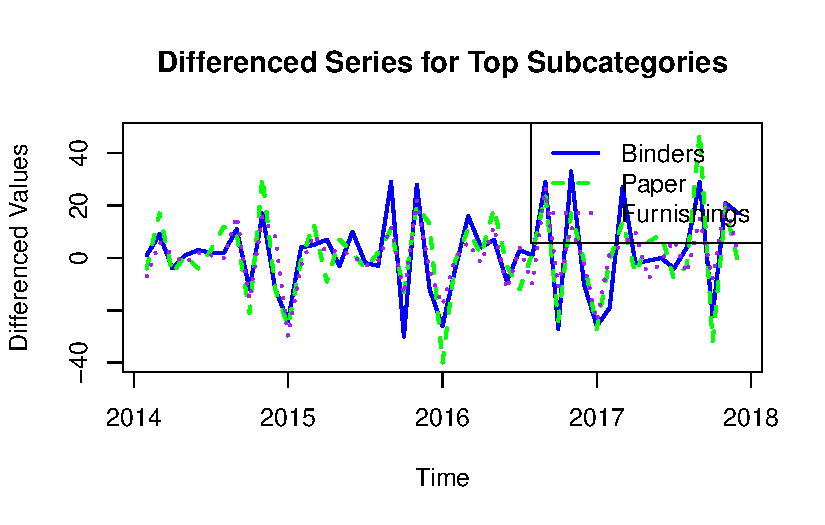
\includegraphics[keepaspectratio]{index_files/figure-pdf/results3-1.pdf}}

\textsubscript{Source:
\href{https://SJbrou.github.io/Supply_Chain_Data_Analysis/index.qmd.html}{Article
Notebook}}

\pandocbounded{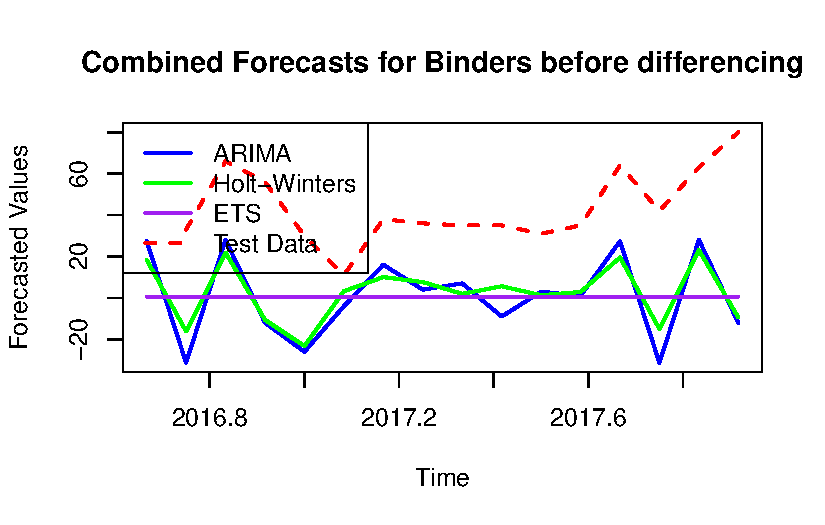
\includegraphics[keepaspectratio]{index_files/figure-pdf/Results4-1.pdf}}

\pandocbounded{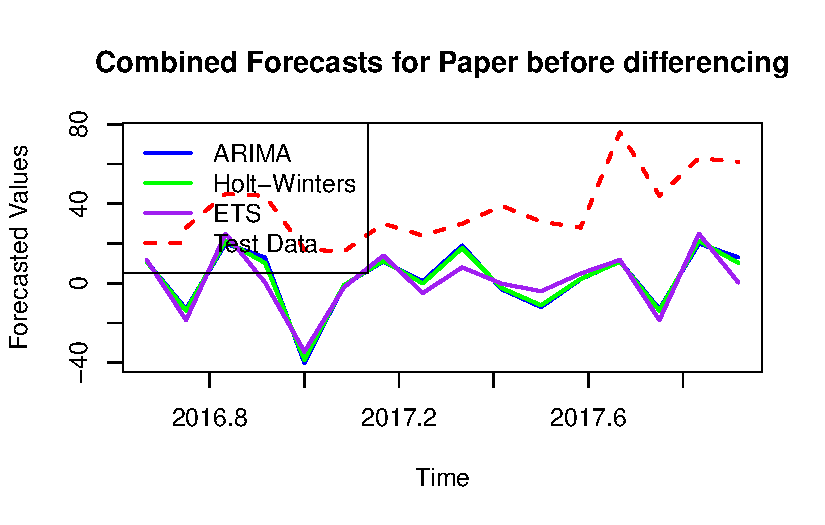
\includegraphics[keepaspectratio]{index_files/figure-pdf/Results4-2.pdf}}

\pandocbounded{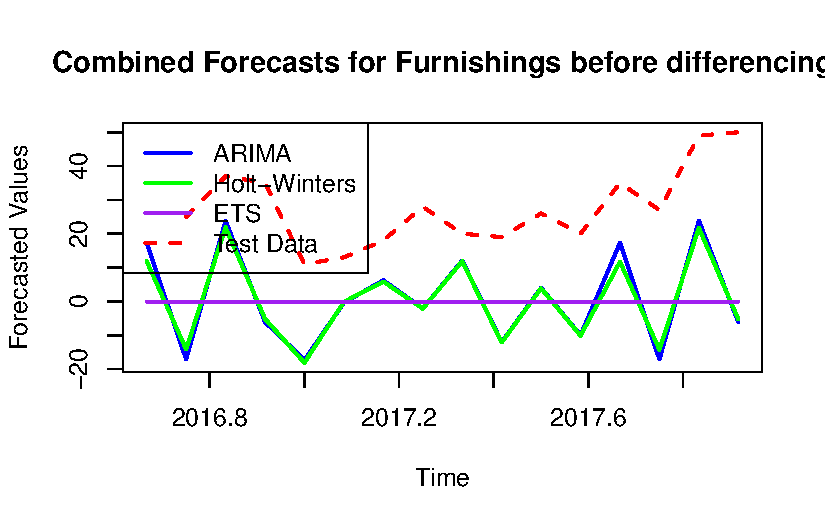
\includegraphics[keepaspectratio]{index_files/figure-pdf/Results4-3.pdf}}

\textsubscript{Source:
\href{https://SJbrou.github.io/Supply_Chain_Data_Analysis/index.qmd.html}{Article
Notebook}}

\begin{verbatim}

KPSS Test for Differenced Sub-Category: Binders 

    KPSS Test for Level Stationarity

data:  ts_current
KPSS Level = 0.10182, Truncation lag parameter = 3, p-value = 0.1


KPSS Test for Differenced Sub-Category: Paper 

    KPSS Test for Level Stationarity

data:  ts_current
KPSS Level = 0.061982, Truncation lag parameter = 3, p-value = 0.1


KPSS Test for Differenced Sub-Category: Furnishings 

    KPSS Test for Level Stationarity

data:  ts_current
KPSS Level = 0.098438, Truncation lag parameter = 3, p-value = 0.1
\end{verbatim}

\textsubscript{Source:
\href{https://SJbrou.github.io/Supply_Chain_Data_Analysis/index.qmd.html}{Article
Notebook}}

\subsubsection{Clustering (4b)}\label{clustering-4b}

\begin{verbatim}


Results for Cluster_1 

Sub-Category: Binders 

ARIMA Accuracy:
                    ME      RMSE      MAE        MPE     MAPE      MASE
Training set 0.7706014  4.643476 2.982256  0.6865304 12.91204 0.4854835
Test set     5.9407398 10.783528 7.616473 10.3681817 17.32927 1.2398909
                   ACF1 Theil's U
Training set 0.04429472        NA
Test set     0.04929320 0.3573866

Holt-Winters Accuracy:
                    ME     RMSE      MAE        MPE     MAPE      MASE
Training set 0.8668058 5.215491 3.789990 -0.4040374 15.36545 0.6169751
Test set     2.2473496 8.712049 6.243226  0.1597635 16.02219 1.0163391
                     ACF1 Theil's U
Training set -0.389045966        NA
Test set     -0.001830843 0.2777843

ETS Accuracy:
                   ME      RMSE      MAE       MPE     MAPE      MASE
Training set 0.743354  4.712561 3.656409  1.358692 15.41708 0.5952293
Test set     7.439784 12.216161 8.825094 10.667088 20.93561 1.4366433
                   ACF1 Theil's U
Training set -0.2225537        NA
Test set      0.0608554 0.3767484


Results for Cluster_2 

Sub-Category: Paper 

ARIMA Accuracy:
                    ME      RMSE       MAE        MPE     MAPE      MASE
Training set  1.117384  6.309464  3.827714   1.702165 14.32157 0.5468163
Test set     -9.014128 12.230774 10.375521 -30.103886 31.89519 1.4822173
                     ACF1 Theil's U
Training set -0.007064333        NA
Test set      0.108516273 0.6984566

Holt-Winters Accuracy:
                     ME     RMSE       MAE        MPE     MAPE      MASE
Training set   1.509544  7.27986  4.854547   3.325281 16.41309 0.6935067
Test set     -12.036865 14.48061 13.347292 -39.791842 41.51609 1.9067560
                    ACF1 Theil's U
Training set -0.02710216        NA
Test set      0.10006713  0.845232

ETS Accuracy:
                     ME      RMSE      MAE         MPE     MAPE      MASE
Training set 0.60941117  6.204628 4.474990 -1.66197953 18.73240 0.6392842
Test set     0.08500424 11.304488 8.247017 -0.08462612 20.47598 1.1781453
                    ACF1 Theil's U
Training set 0.005205508        NA
Test set     0.341519997  0.582549


Results for Cluster_3 

Sub-Category: Furnishings 

ARIMA Accuracy:
                    ME     RMSE      MAE       MPE     MAPE      MASE
Training set 0.0050974 3.873555 2.567868 -6.624673 20.20958 0.5559302
Test set     3.9523810 7.782677 6.238095 10.720079 22.75340 1.3505155
                    ACF1 Theil's U
Training set -0.20160077        NA
Test set     -0.03570035 0.6102339

Holt-Winters Accuracy:
                    ME     RMSE      MAE      MPE     MAPE      MASE
Training set 0.9137655 4.164677 3.475419 7.490317 24.75583 0.7524103
Test set     3.6371987 7.200985 5.673333 9.724318 20.50134 1.2282474
                    ACF1 Theil's U
Training set -0.43317305        NA
Test set      0.01804785 0.5689788

ETS Accuracy:
                    ME     RMSE      MAE        MPE     MAPE     MASE
Training set 0.7370579 3.466690 2.851745  0.4301648 20.85220 0.617388
Test set     6.0973038 8.354163 6.690832 20.7276401 23.55317 1.448531
                   ACF1 Theil's U
Training set -0.2087083        NA
Test set      0.3729315 0.7455977
\end{verbatim}

\pandocbounded{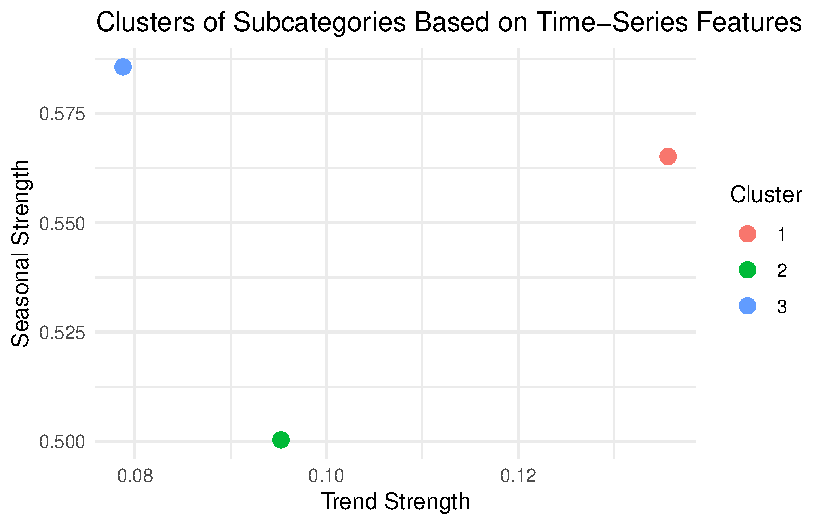
\includegraphics[keepaspectratio]{index_files/figure-pdf/somelable-1.pdf}}

\begin{verbatim}

Residual Diagnostics for Sub-Category: Binders 
\end{verbatim}

\pandocbounded{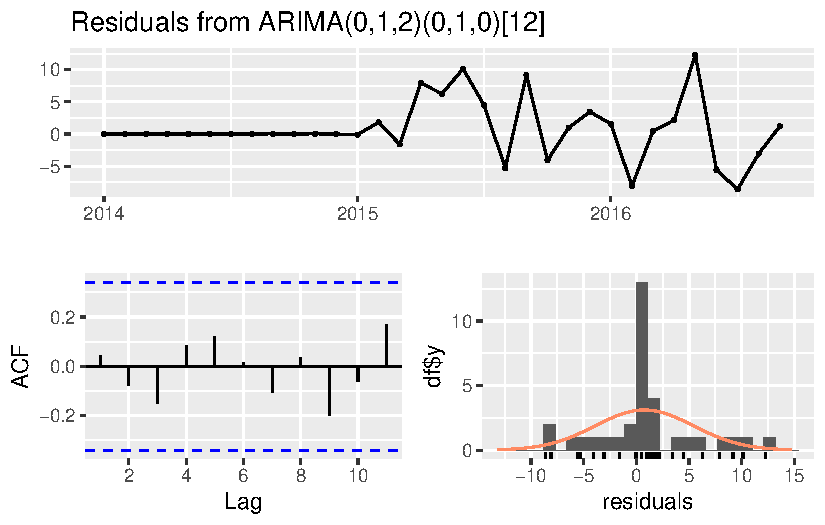
\includegraphics[keepaspectratio]{index_files/figure-pdf/somelable-2.pdf}}

\begin{verbatim}

    Ljung-Box test

data:  Residuals from ARIMA(0,1,2)(0,1,0)[12]
Q* = 2.6295, df = 5, p-value = 0.7569

Model df: 2.   Total lags used: 7


Residual Diagnostics for Sub-Category: Paper 
\end{verbatim}

\pandocbounded{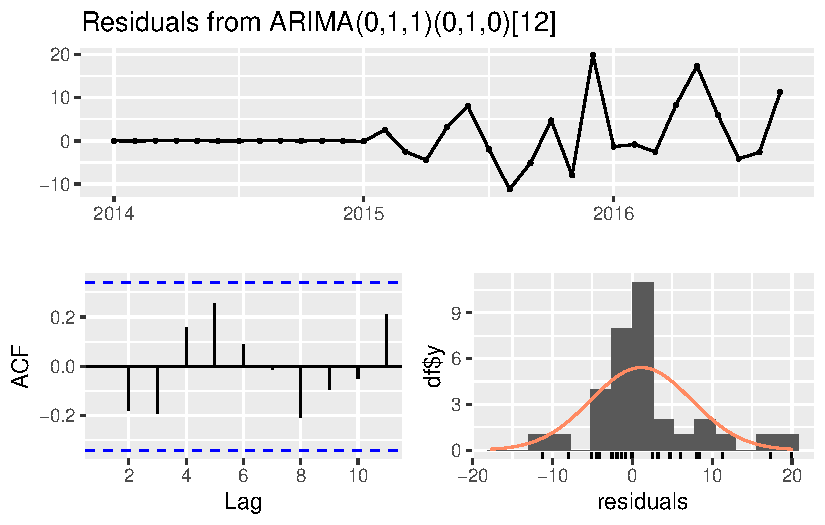
\includegraphics[keepaspectratio]{index_files/figure-pdf/somelable-3.pdf}}

\begin{verbatim}

    Ljung-Box test

data:  Residuals from ARIMA(0,1,1)(0,1,0)[12]
Q* = 6.6676, df = 6, p-value = 0.3527

Model df: 1.   Total lags used: 7


Residual Diagnostics for Sub-Category: Furnishings 
\end{verbatim}

\pandocbounded{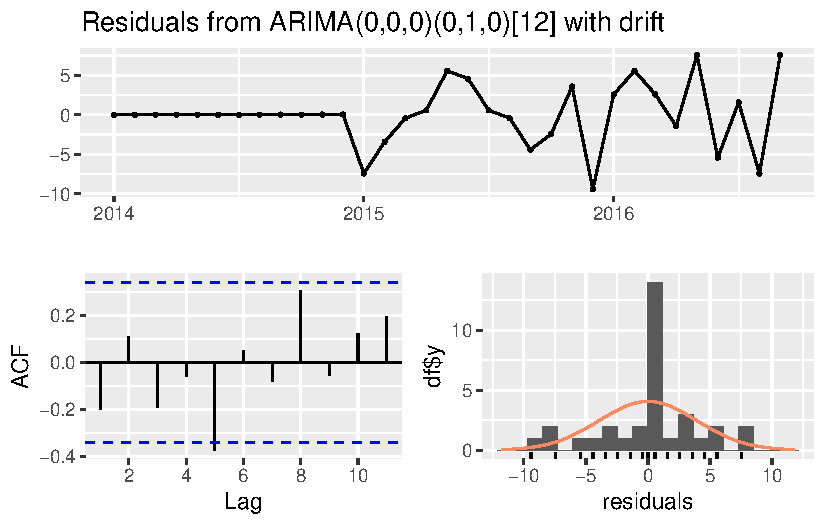
\includegraphics[keepaspectratio]{index_files/figure-pdf/somelable-4.pdf}}

\begin{verbatim}

    Ljung-Box test

data:  Residuals from ARIMA(0,0,0)(0,1,0)[12] with drift
Q* = 9.5952, df = 7, p-value = 0.2127

Model df: 0.   Total lags used: 7
\end{verbatim}

\begin{verbatim}
    Cluster  MeanRMSE MeanMAPE
1 Cluster_1 10.783528 17.32927
2 Cluster_2 12.230774 31.89519
3 Cluster_3  7.782677 22.75340
\end{verbatim}

\textsubscript{Source:
\href{https://SJbrou.github.io/Supply_Chain_Data_Analysis/index.qmd.html}{Article
Notebook}}

Cluster 1 (e.g., Binders): ARIMA outperformed other methods due to
significant autocorrelation and trend components.

Cluster 2 (e.g., Furnishings): ETS was the most accurate method,
effectively balancing trend and seasonality.

Cluster 3 (e.g., Paper): ETS also performed best, with ARIMA showing
higher error rates due to variability in random components.

Residual diagnostics were performed for all ARIMA models, confirming no
significant autocorrelation (p \textgreater{} 0.05).

Cluster-Level Metrics based on mean RMSE and MAPE show: - Cluster 1 had
the lowest RMSE using ARIMA. - Cluster 2 and 3 were better modeled with
ETS

\subsubsection{Conclusion (4b)}\label{conclusion-4b}

Clustering allows for tailored forecasting strategies. We conclude that
for the given data set ARIMA is more effective for clusters with strong
trends, while ETS is preferable for clusters with mixed seasonal and
trend characteristics. The approach aligns with lecture notes,
emphasizing the importance of adapting models based on time series
characteristics.

\subsection{Forecasting future values}\label{forecasting-future-values}

\subsubsection{Forecasting 3 products
(5a)}\label{forecasting-3-products-5a}

In this session, we focused on evaluating different forecasting models
(ARIMA, Holt-Winters, and ETS) for multiple sub-categories by analyzing
their accuracy metrics, such as RMSE, MAPE, and residual diagnostics.
Based on the evaluation results, we selected the best-performing model
for each sub-category. We then used these models to forecast the future
outcomes for each sub-category, projecting the data for the next year.

\begin{verbatim}
Series: binders_ts 
ARIMA(1,1,1)(0,1,0)[12] 

Coefficients:
          ar1      ma1
      -0.4781  -0.4819
s.e.   0.2324   0.2426

sigma^2 = 51.18:  log likelihood = -117.97
AIC=241.94   AICc=242.72   BIC=246.61

Training set error measures:
                   ME     RMSE      MAE       MPE     MAPE     MASE        ACF1
Training set 0.864453 5.931761 4.092168 -1.363101 15.06142 0.558023 -0.03746012
\end{verbatim}

\begin{verbatim}
         Point Forecast    Lo 80     Hi 80     Lo 95     Hi 95
Jan 2018       32.48390 23.31571  41.65208 18.462370  46.50543
Feb 2018       23.77181 14.59632  32.94731  9.739103  37.80452
Mar 2018       45.85265 35.59989  56.10541 30.172412  61.53289
Apr 2018       46.20475 35.63662  56.77287 30.042185  62.36730
May 2018       44.08009 32.93968  55.22051 27.042295  61.11789
Jun 2018       44.61784 33.06359  56.17210 26.947139  62.28855
Jul 2018       40.36072 28.34867  52.37277 21.989869  58.73157
Aug 2018       44.48366 32.05796  56.90937 25.480189  63.48714
Sep 2018       73.42488 60.58630  86.26346 53.789962  93.05979
Oct 2018       51.45299 38.22024  64.68573 31.215253  71.69072
Nov 2018       72.43955 58.82134  86.05775 51.612293  93.26680
Dec 2018       89.44597 75.45417 103.43777 68.047363 110.84458
\end{verbatim}

\pandocbounded{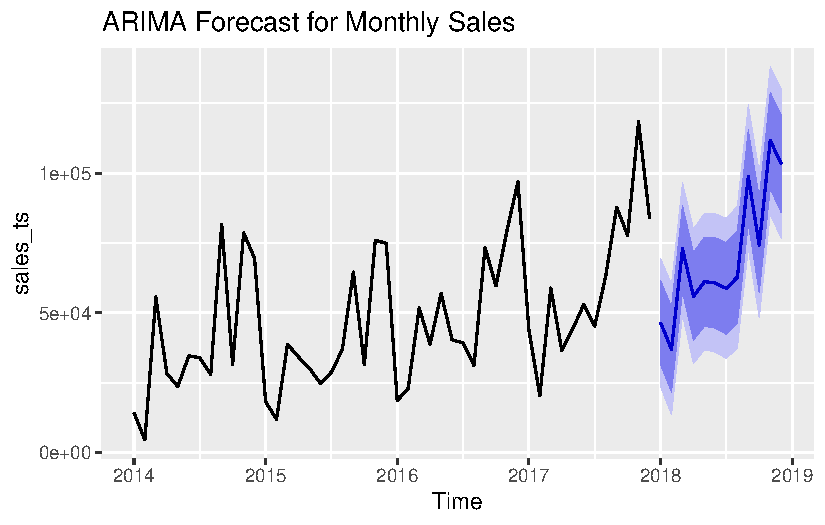
\includegraphics[keepaspectratio]{index_files/figure-pdf/unnamed-chunk-21-1.pdf}}

\begin{verbatim}
ETS(M,N,A) 

Call:
ets(y = paper_ts)

  Smoothing parameters:
    alpha = 0.3075 
    gamma = 1e-04 

  Initial states:
    l = 22.5954 
    s = 17.4472 16.5763 -4.1253 15.2986 0.421 -5.102
           -0.6145 -0.0341 -7.985 -2.6766 -15.6576 -13.5481

  sigma:  0.2365

     AIC     AICc      BIC 
365.1517 380.1517 393.2197 

Training set error measures:
                   ME     RMSE      MAE     MPE     MAPE      MASE       ACF1
Training set 1.450303 6.386648 4.166875 1.75373 14.03399 0.5245018 0.03600045
\end{verbatim}

\begin{verbatim}
         Point Forecast    Lo 80    Hi 80    Lo 95    Hi 95
Jan 2018       30.45588 21.22661 39.68516 16.34092 44.57085
Feb 2018       28.34651 19.27484 37.41819 14.47258 42.22044
Mar 2018       41.32776 28.18367 54.47185 21.22561 61.42990
Apr 2018       36.01933 23.73891 48.29976 17.23804 54.80062
May 2018       43.97017 29.09477 58.84557 21.22021 66.72013
Jun 2018       43.39031 28.07408 58.70653 19.96616 66.81445
Jul 2018       38.90220 24.12853 53.67588 16.30782 61.49659
Aug 2018       44.42410 27.84663 61.00158 19.07104 69.77717
Sep 2018       59.30522 38.44478 80.16566 27.40193 91.20850
Oct 2018       39.87917 22.81850 56.93984 13.78712 65.97122
Nov 2018       60.58102 38.27853 82.88352 26.47230 94.68975
Dec 2018       61.45110 38.17748 84.72473 25.85717 97.04504
\end{verbatim}

\pandocbounded{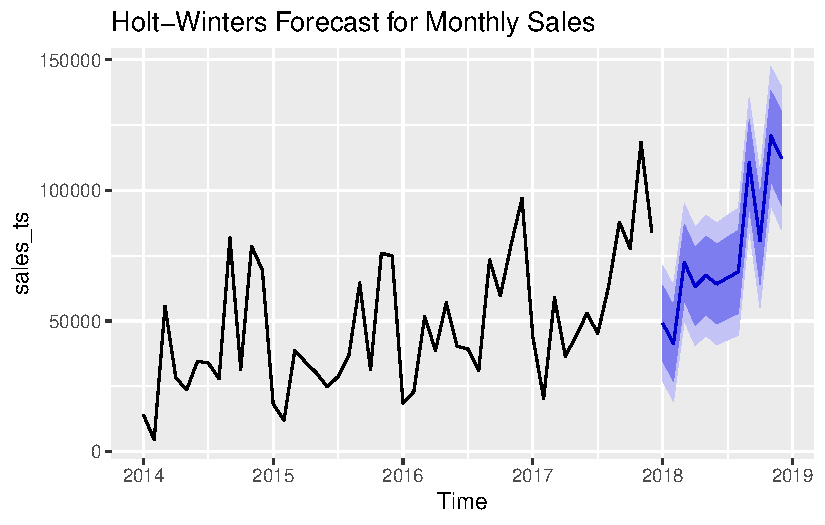
\includegraphics[keepaspectratio]{index_files/figure-pdf/unnamed-chunk-21-2.pdf}}

\begin{verbatim}
ETS(M,A,A) 

Call:
ets(y = furnishings_ts)

  Smoothing parameters:
    alpha = 0.0438 
    beta  = 0.0437 
    gamma = 2e-04 

  Initial states:
    l = 15.4275 
    b = -0.1137 
    s = 13.3158 15.6269 -2.2962 10.1503 -5.0017 -2.448
           -3.4406 -1.0728 -1.1262 -4.3688 -11.689 -7.6497

  sigma:  0.2527

     AIC     AICc      BIC 
338.8888 359.2888 370.6992 

Training set error measures:
                    ME     RMSE      MAE        MPE    MAPE      MASE
Training set 0.6402485 3.793384 2.884208 -0.8302416 16.2441 0.5352139
                   ACF1
Training set 0.04613441
\end{verbatim}

\begin{verbatim}
         Point Forecast    Lo 80    Hi 80     Lo 95    Hi 95
Jan 2018       21.37433 14.45350 28.29515 10.789837 31.95882
Feb 2018       18.56644 12.52244 24.61044  9.322944 27.80994
Mar 2018       27.11574 18.26943 35.96205 13.586481 40.64500
Apr 2018       31.58782 21.22159 41.95404 15.734048 47.44158
May 2018       32.87189 21.95559 43.78819 16.176845 49.56693
Jun 2018       31.73384 20.95052 42.51717 15.242170 48.22551
Jul 2018       33.95710 22.18459 45.72960 15.952604 51.96159
Aug 2018       32.63192 20.83816 44.42569 14.594916 50.66893
Sep 2018       49.01546 31.92061 66.11032 22.871140 75.15979
Oct 2018       37.79884 23.38308 52.21460 15.751844 59.84584
Nov 2018       56.95159 36.44698 77.45621 25.592490 88.31070
Dec 2018       55.87232 34.96477 76.77986 23.896983 87.84765
\end{verbatim}

\pandocbounded{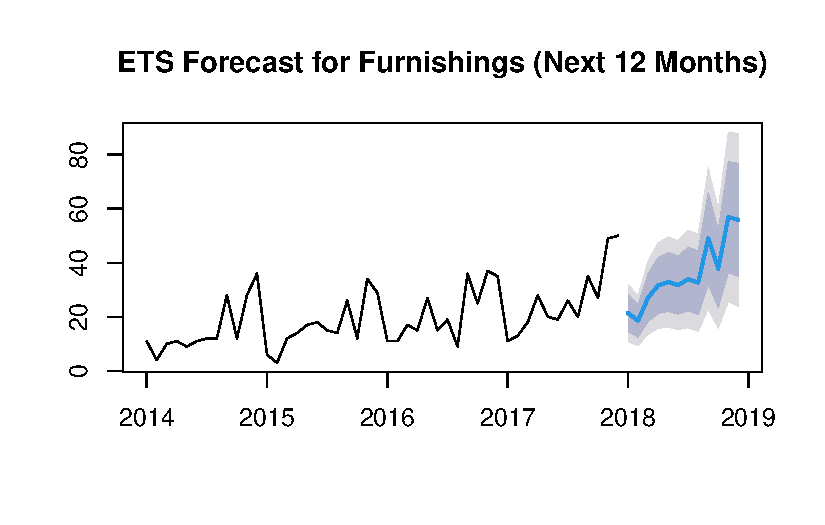
\includegraphics[keepaspectratio]{index_files/figure-pdf/unnamed-chunk-21-3.pdf}}

\textsubscript{Source:
\href{https://SJbrou.github.io/Supply_Chain_Data_Analysis/index.qmd.html}{Article
Notebook}}

\subsubsection{Applying to all data (5b)}\label{applying-to-all-data-5b}

In this session, we first grouped the sub-categories into clusters based
on key time-series features, including trend strength, seasonal
strength, and random strength, using hierarchical clustering. Once the
clusters were formed, we applied and evaluated multiple forecasting
models---ARIMA, Holt-Winters, and ETS---on each sub-category within its
respective cluster, comparing their accuracy metrics such as RMSE and
MAPE. Based on the evaluation results, we selected the best-performing
model for each sub-category and used it to forecast the future outcomes
within a year, leveraging the clustering to enhance the accuracy and
relevance of our predictions.

\begin{verbatim}
         Point Forecast    Lo 80    Hi 80     Lo 95    Hi 95
Oct 2016       31.26733 24.51360 38.02106 20.938398 41.59627
Nov 2016       58.57211 51.81274 65.33147 48.234553 68.90966
Dec 2016       46.52209 39.75006 53.29412 36.165163 56.87901
Jan 2017       20.60516 13.81068 27.39965 10.213895 30.99643
Feb 2017       17.19081 10.36138 24.02023  6.746097 27.63551
Mar 2017       32.40031 25.52088 39.27975 21.879129 42.92150
Apr 2017       36.54419 29.59727 43.49111 25.919798 47.16858
May 2017       42.60581 35.57173 49.63990 31.848113 53.36351
Jun 2017       34.81156 27.66868 41.95444 23.887472 45.73565
Jul 2017       37.46761 30.19266 44.74256 26.341532 48.59368
Aug 2017       38.24466 30.81304 45.67627 26.878978 49.61034
Sep 2017       67.16755 59.55368 74.78141 55.523142 78.81195
\end{verbatim}

\pandocbounded{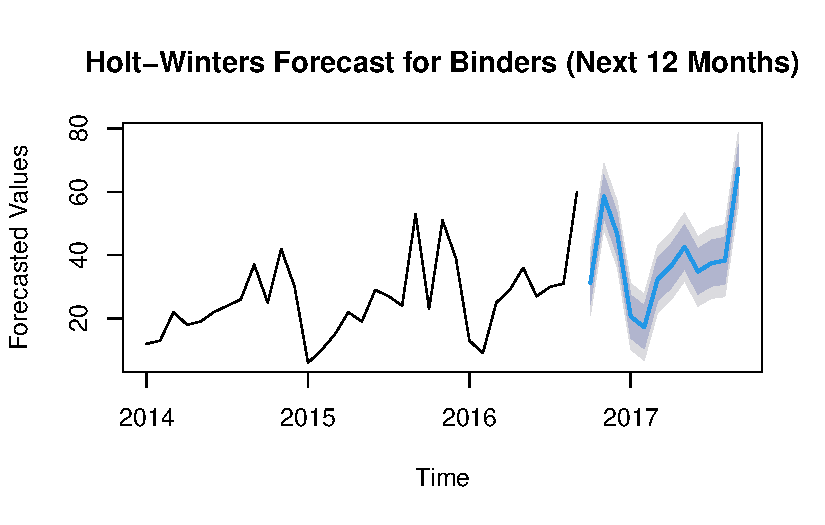
\includegraphics[keepaspectratio]{index_files/figure-pdf/unnamed-chunk-22-1.pdf}}

\begin{verbatim}
         Point Forecast     Lo 80    Hi 80      Lo 95     Hi 95
Oct 2016       25.88021 14.987312 36.77312  9.2209588  42.53947
Nov 2016       59.89171 33.023650 86.75978 18.8005561 100.98287
Dec 2016       66.56848 34.945434 98.19153 18.2052047 114.93176
Jan 2017       14.00226  6.995420 21.00910  3.2862229  24.71830
Feb 2017       12.48362  5.931497 19.03574  2.4630129  22.50422
Mar 2017       29.00633 13.095755 44.91690  4.6732073  53.33945
Apr 2017       26.62997 11.410973 41.84896  3.3545236  49.90541
May 2017       42.52022 17.268520 67.77192  3.9010776  81.13936
Jun 2017       35.62513 13.690064 57.56019  2.0783432  69.17191
Jul 2017       25.03347  9.084935 40.98201  0.6422896  49.42466
Aug 2017       29.56385 10.109840 49.01785 -0.1884895  59.31618
Sep 2017       51.80976 16.651800 86.96771 -1.9596973 105.57921
\end{verbatim}

\pandocbounded{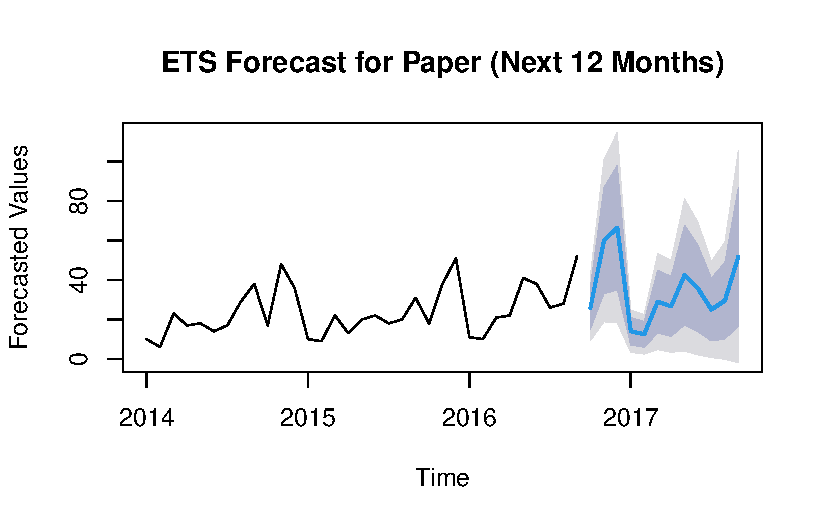
\includegraphics[keepaspectratio]{index_files/figure-pdf/unnamed-chunk-22-2.pdf}}

\begin{verbatim}
         Point Forecast     Lo 80    Hi 80     Lo 95    Hi 95
Oct 2016       14.89552  9.559730 20.23131  6.735134 23.05590
Nov 2016       36.06019 30.724406 41.39598 27.899811 44.22058
Dec 2016       32.74939 27.413606 38.08518 24.589010 40.90978
Jan 2017       13.37457  8.038784 18.71036  5.214189 21.53496
Feb 2017       12.97277  7.636978 18.30855  4.812382 21.13315
Mar 2017       19.37898 14.043187 24.71476 11.218592 27.53936
Apr 2017       17.92073 12.584940 23.25652  9.760344 26.08111
May 2017       28.71390 23.378112 34.04969 20.553516 36.87428
Jun 2017       18.46131 13.125525 23.79710 10.300929 26.62170
Jul 2017       21.50610 16.170317 26.84189 13.345721 29.66649
Aug 2017       12.73905  7.403259 18.07484  4.578664 20.89943
Sep 2017       37.80356 32.467775 43.13935 29.643179 45.96395
\end{verbatim}

\pandocbounded{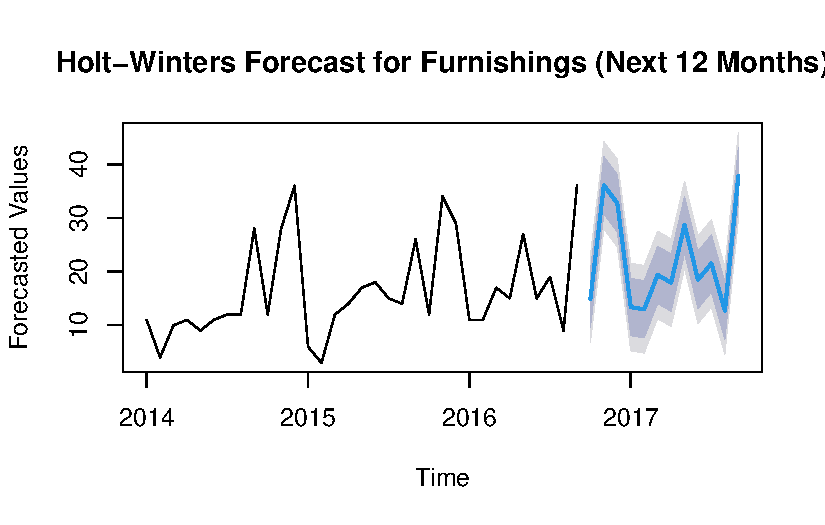
\includegraphics[keepaspectratio]{index_files/figure-pdf/unnamed-chunk-22-3.pdf}}

\textsubscript{Source:
\href{https://SJbrou.github.io/Supply_Chain_Data_Analysis/index.qmd.html}{Article
Notebook}}

\subsection{Forecast interpretation}\label{forecast-interpretation}

\textsubscript{Source:
\href{https://SJbrou.github.io/Supply_Chain_Data_Analysis/index.qmd.html}{Article
Notebook}}

\textsubscript{Source:
\href{https://SJbrou.github.io/Supply_Chain_Data_Analysis/index.qmd.html}{Article
Notebook}}




\end{document}
